\section{Introduction}
\subsection{Équipe}
\begin{frame}
    \frametitle{\color{white}Équipe}
  \begin{center}
    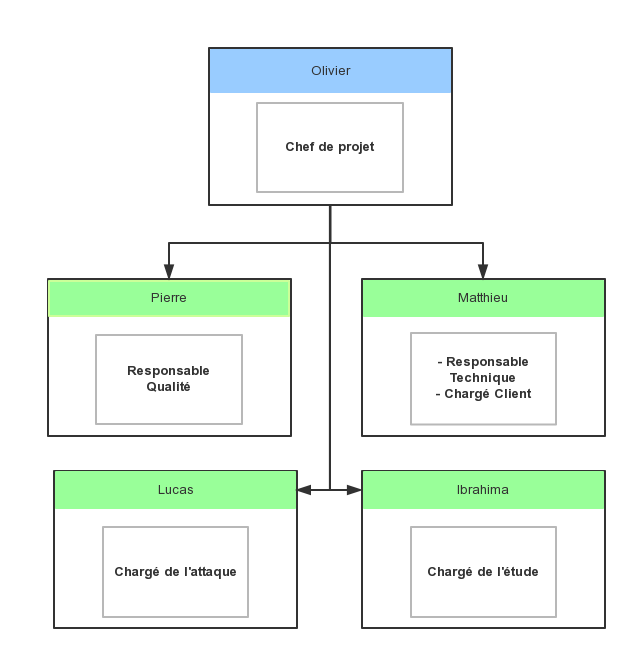
\includegraphics[scale=0.30]{guipgteam.png}
  \end{center}
\end{frame}
% 
\subsection{PGP}
\begin{frame}
    \frametitle{\color{white}PGP}
    \begin{block}{Qu'est ce que PGP ?}
    	\begin{itemize}
    	 \item Logiciel créé par Phil Zimmermann en 1991.
         \item Pretty Good Privacy = Assez bonne confidentialité
       \end{itemize} 
    \end{block}
    \begin{block}{Pourquoi ?}
    	\begin{itemize}
         \item Permettre l'utilisation de la cryptographie pour le grand public
         \item Chiffrer, déchiffrer, signer et vérifier des données. 
       \end{itemize} 
    \end{block}
\end{frame}
\begin{frame}
    \frametitle{\color{white}PGP}
    \begin{block}{Comment ?}
    	\begin{itemize}
         \item Utilisation de cryptographie hybride = sysmétrique + asymétrique
         \item Un utilisateur doit posséder:
	  \begin{itemize}
	    \item Sa propre paire de clefs asymétriques (privée et public).
	    \begin{itemize}
	      \item La clef privée sert à signer et déchiffrer.
	      \item La clef publique sert à chiffrer et vérifier.
	    \end{itemize}
	    \item Les clefs publiques des personnes avec qui il souhaite communiquer.
	    \begin{itemize}
	      \item Pour chiffrer des données qui leurs sont déstinées.
	      \item Pour vérifier des données qu'ils ont signé.
	    \end{itemize}
	  \end{itemize}
	  \item Les données sont chiffrées ou déchiffrées par clef symétrique.
	  \item Les clefs symétriques utilisées sont chiffrées ou déchiffrées par les clefs asymétriques des utilisateurs.
       \end{itemize} 
    \end{block}
\end{frame}

\begin{frame}
    \frametitle{\color{white}PGP}
    \begin{block}{Qu'est ce qu'une clef PGP ?}
    	\begin{itemize}
	  \item Une clef asymétrique privée ou publique.
	  \item Une date de création.
	  \item Une empreinte ( = le hashé de la clef + la date de création)
	  \item Un utilisateur (nom et adresse email).
	  \item Une auto-signature (faite par cette même clef).
	  \item Un niveau de validité.
	  \item Un niveau de confiance.
       \end{itemize} 
    \end{block}
\end{frame}

\subsection{OpenPGP}
\begin{frame}
    \frametitle{\color{white}OpenPGP}
    \begin{block}{Qu'est ce que OpenPGP ?}
    	\begin{itemize}
    	 \item Crée en 1997 par l'IETF (Internet Engineering Task Force)
    	 \item Protocol libre permettant de sécuriser l'échange d'email.
    	 \item Définit différents formats de paquets (message chiffré, signature, clef privée, clef publique...).
    	 \item Se base sur le logiciel PGP.
         \item Aujourd'hui normalisé dans la RFC 4880.
       \end{itemize} 
    \end{block}
\end{frame}

\subsection{GnuPG}
\begin{frame}
    \frametitle{\color{white}GPG}
    \begin{block}{Qu'est ce que GPG ?}
      \begin{itemize}
        \item GnuPG = GNU Privacy Guard
        \item Logiciel libre crée par Werner KOCH en 1997.
        \item Basé sur le standard OpenPGP.
        \item Remplacer PGP.
      \end{itemize}
    \end{block}
\end{frame}